\documentclass{article}

% if you need to pass options to natbib, use, e.g.:
%     \PassOptionsToPackage{numbers, compress}{natbib}
% before loading neurips_2019

% ready for submission
% \usepackage{neurips_2019}

% to compile a preprint version, e.g., for submission to arXiv, add add the
% [preprint] option:
%     \usepackage[preprint]{neurips_2019}

% to compile a camera-ready version, add the [final] option, e.g.:
     \usepackage[final]{neurips_2019}

% to avoid loading the natbib package, add option nonatbib:
%     \usepackage[nonatbib]{neurips_2019}

\usepackage[utf8]{inputenc} % allow utf-8 input
\usepackage[T1]{fontenc}    % use 8-bit T1 fonts
\usepackage{hyperref}       % hyperlinks
\usepackage{url}            % simple URL typesetting
\usepackage{booktabs}       % professional-quality tables
\usepackage{amsfonts}       % blackboard math symbols
\usepackage{nicefrac}       % compact symbols for 1/2, etc.
\usepackage{microtype}      % microtypography

\usepackage{graphicx} 
\usepackage{float}
\usepackage{subfigure}

\title{MAFS6010Z Artificial Intelligence in Fintech \\ Project 1}

% The \author macro works with any number of authors. There are two commands
% used to separate the names and addresses of multiple authors: \And and \AND.
%
% Using \And between authors leaves it to LaTeX to determine where to break the
% lines. Using \AND forces a line break at that point. So, if LaTeX puts 3 of 4
% authors names on the first line, and the last on the second line, try using
% \AND instead of \And before the third author name.

\author{%
  CHAN Koon Lam 20748995 \AND LAM Chung Wai 20430732 \AND TANG Tsz Hong 20735194

  % examples of more authors
  % \And
  % Coauthor \\
  % Affiliation \\
  % Address \\
  % \texttt{email} \\
  % \AND
  % Coauthor \\
  % Affiliation \\
  % Address \\
  % \texttt{email} \\
  % \And
  % Coauthor \\
  % Affiliation \\
  % Address \\
  % \texttt{email} \\
  % \And
  % Coauthor \\
  % Affiliation \\
  % Address \\
  % \texttt{email} \\
}

\begin{document}
\maketitle
\section{Kaggle Contest: Home Credit Default Risk}
As a warm-up task about machine learning, we focused on the "Home Credit Default Risk" problem on Kaggle. (\url{https://www.kaggle.com/c/home-credit-default-risk/}) Home Credit is an international financial institution that specialized in consumer loans and personal loans. In the Kaggle contest, we are trying to predict if the applicant is the company's target with 8 data files and more than 120 predictors.

The following article includes Data Cleaning, Data Visualization, Modelling with different techniques, and evaluation with ROC, AUC. We obtained 0.739 score on Kaggle contest. The proof is in Appendix II.

\section{Data Preprocessing}

\subsection{Data Description}

In the problem, there are 8 different data files. 

\begin{itemize}

\item application\_train.csv  \& application\_test.csv \\
\\
This is the main data set. The shape of the data frame is (307507, 122). It contains the output "TARGET", the ID of loan, and 120 predictors that are related to the personal information of the client. \\

details of some important columns: \\
 "TARGET"- it means client with payment difficulties, the definition of late payment is he/she had late payment more than X days on at least one of the first Y installments of the loan in our sample. \\

\item bureau.csv  \& bureau\_balance.csv \\

This is the previous credits records in the credit bureau. In these dataset, we can know about the previous credit record of client and the current status of the Credit Bureau loan. \\

details of some important columns: \\
"STATUS" - C means closed, X means status unknown, 0 means no DPD (days past due), 1 means 1-30 DPD, 2 means 31-60 DPD, ... , 5 means 120+ or sold or written off 
DPD 
\\

\item previous\_application.csv \\
 credit\_card\_balance.csv \& POS\_CASH\_balance.csv \& installments\_payments.csv \\

This is the previous credit record in Home credit. "NAME\_CONTRACT\_TYPE" subdivides the record into three types, credit card, POS cash and instalments payments. More record details are stored in the corresponding csv files. \\


\end{itemize}

\subsection{Data Cleaning and Interpretation}

\paragraph{Dealing with NaN values} \mbox{}

Some data contain NaN values. There are several approaches, we can either drop the data, drop the predictor, or use an appropriate approach e.g., use 0 to fill the values back and then add columns to indicate the existence of missing values (i.e. add a column “COMMANAREA\_NA” to indicate whether the “COMMANAREA” has missing value).	

We plot the NaN values in the application train, slot them in descending order of percentage. The predictive power of these features would be low.


\begin{figure}[H]
  \centering
  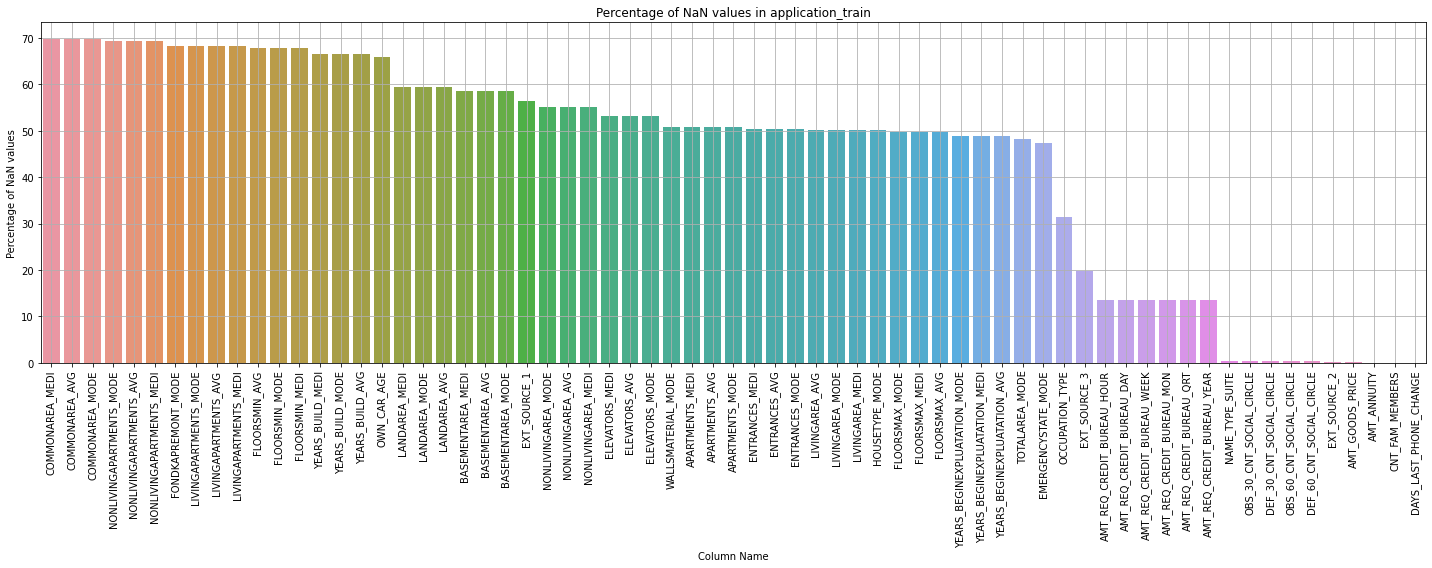
\includegraphics [width=14cm]{download1.png}
  \caption{Percentage of NaN values in application train}
\end{figure}

\paragraph{Features} \mbox{}

We also tried to visualize the data, to see if there exists some important insight. By Figure 2, we understand the outputs are mostly 0, we have to avoid the model generating all 0 as prediction. By Figure 3, it shows how different predictors affect the TARGET. We are guessing days\_birth, ext\_source\_1, ext\_source\_2 , ext\_source\_3 are important features to the model, as they have significantly different curve on different TARGET output.

\begin{figure}[H]
  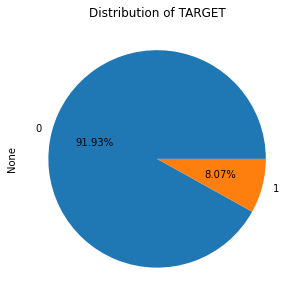
\includegraphics [width=4cm]{download2.png}
  \caption{Distribution of TARGET}
\end{figure}

\begin{figure}[H]
  \centering
  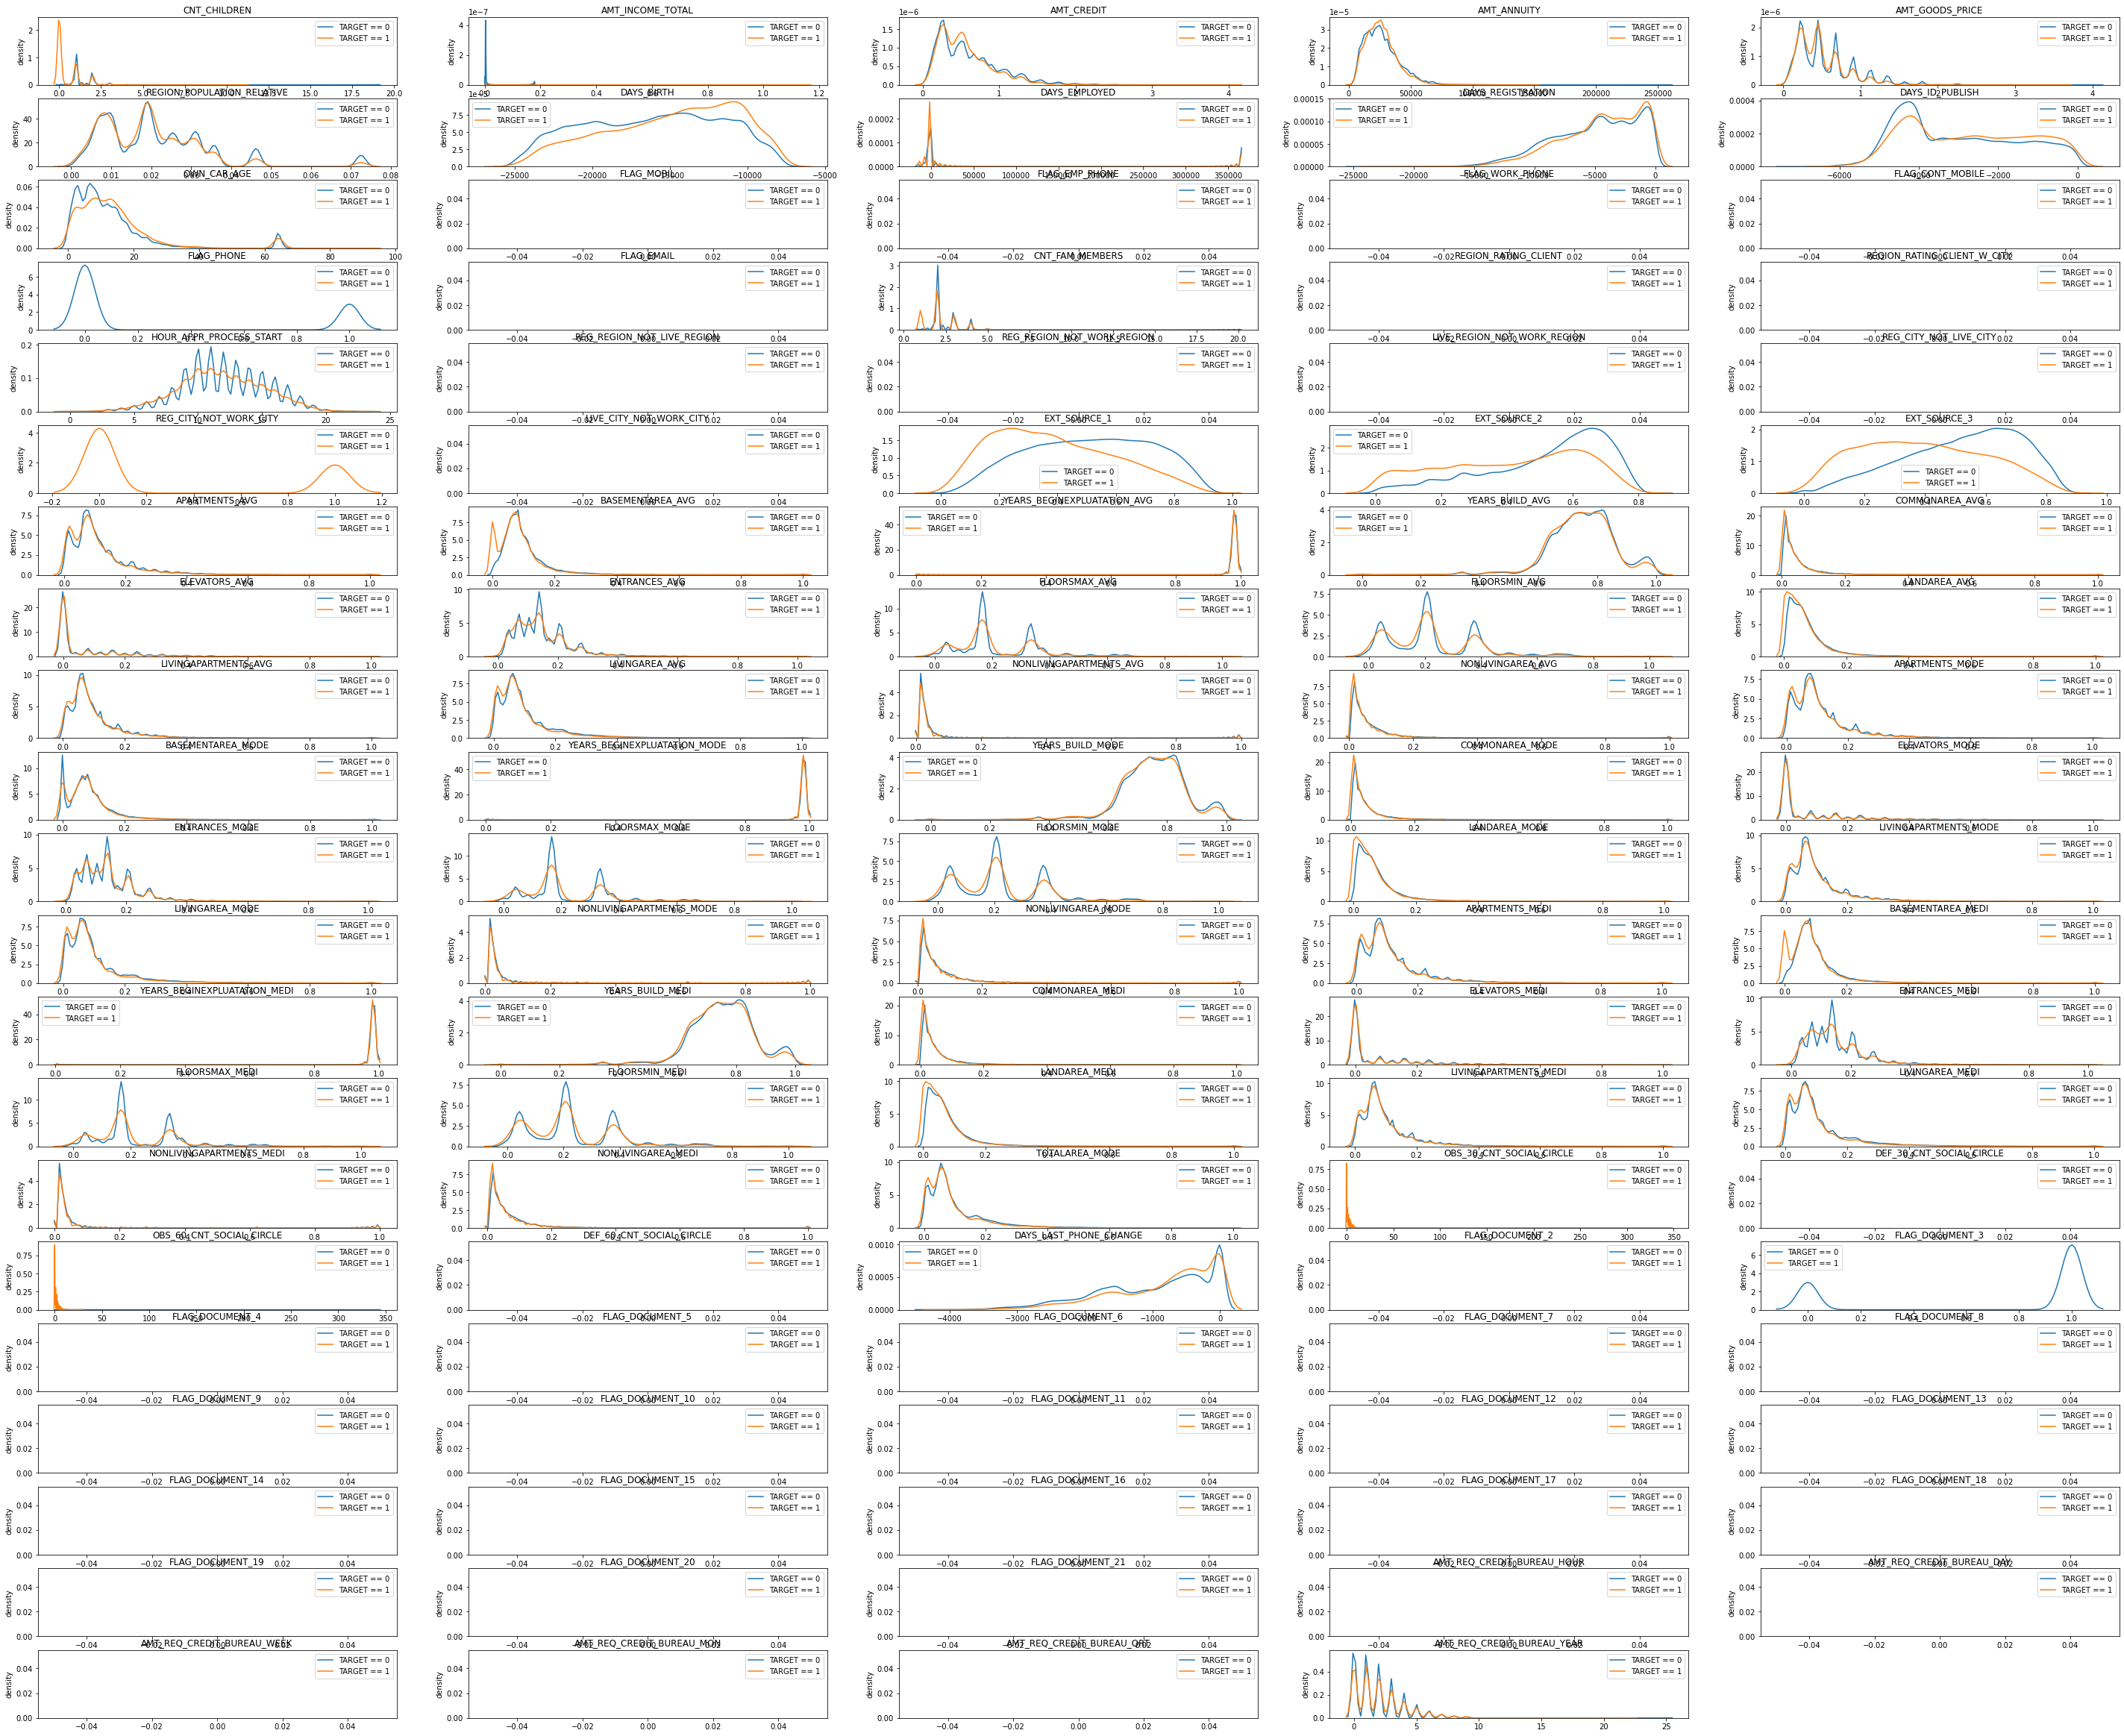
\includegraphics [width=14cm]{download3.png}
  %\fbox{\rule[-.5cm]{0cm}{4cm} \rule[-.5cm]{4cm}{0cm}}
  \caption{The plot of how different predictors affecting the TARGET. (zoom in to see details).}
\end{figure}


\paragraph{Oversampling} \mbox{}

We have used oversampling on the training data to duplicate examples in the minority class. This is because the dataset is severely imbalanced which could cause the algorithm to ignore the minority class. This is effective in iterative learning models such as xgBoost and random forests.

\mbox{}

\section{Models and Evaluations}



\subsection{Models}

As the output "TARGET" is a binary output, we have tried different classification approaches and compared their performance.
We have fitted classification algorithms like Logistic Regression, Decision Tree, Random Forest, Linear Discriminant Analysis, K-nearest neighbours, Gradient Boosting; also tested 2 commonly used gradient boosting frameworks in machine learning community, XGBoost and LightGBM.
		
\newpage
			
The methodology is as follows. The dataset application\_train.csv is divided into training set and validation set. Then we fit the training set into different models. Finally, we will choose the best model, using the data from application\_test.csv to get predictions, and upload it to Kaggle to get the Kaggle score. By the below result, XGBoost performs the best among all.

\mbox{}

\begin{table}[H]
  \caption{models}
  \label{sample-table}
  \centering
  \begin{tabular}{lll}
    \toprule
    \multicolumn{2}{c}{}                   \\
    %\cmidrule(r){1-2}
    Name   &  Computation Time & AUC (in validation set)   \\
    \midrule
    Logistic Regression & 8s & 0.63   \\
    Decision Tree & 8s & 0.69  \\
    Random Forest & 1min 3s & 0.73 \\
    Linear Discriminant Analysis & 14s & 0.74 \\
    K-nearest neighbours & 20s & 0.56 \\
    Gradient Boosting & 4min 50s & 0.75 \\
    XGBoost & 50s & 0.75 \\
    LightGBM & 1min 40s & 0.74 \\
    \bottomrule
  \end{tabular}
\end{table}

\mbox{}

\subsection{ROC AUC}

To evaluate the models’ performance, we often use the ROC curve. ROC curve (Receiver Operating Characteristic Curve) is the curve that plots True Positive Rate against False Positive Rate. AUC means Area under curve. AUC=0.5 means the model has no discrimination power. We often consider >0.7 AUC as a good model, >0.8 AUC as an excellent model.		

The below shows the ROC curve and its AUC of the different models.


\begin{figure}[H]
  \centering
  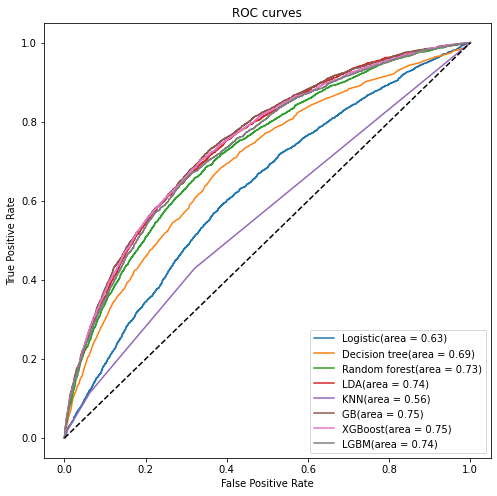
\includegraphics [width=8cm]{download4.png}
  \caption{Plot of different ROC curve of different models}
\end{figure}

\newpage


\section{Conclusion}

We believe the XGBoost model can best predict TARGET for this Home Credit Default Risk problem. It has AUC=0.75 in validation set and Kaggle score 0.739.		
	
Because of computation time, we did not include all the sub dataset as the feature of the model. More in-depth investigation can be made in future analysis.

Within the XGBoost model, we found out that the following variables have the highest relative importance in affecting the output. The most important features shown in order are EXT\_SOURCE\_2, EXT\_SOURCE\_3, DAYS\_BIRTH, DAYS\_ID\_PUBLISH and AMT\_ANNUITY, which has similar insight when we visualize the features.

\begin{figure}[H]
  \centering
  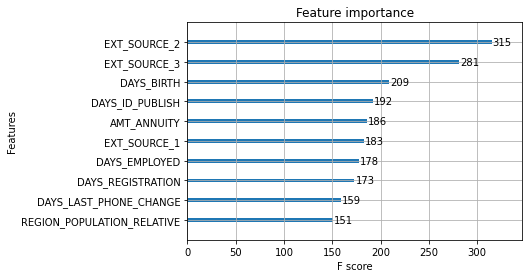
\includegraphics [width=10cm]{download6.png}
  \caption{Feature importantce}
\end{figure}

\newpage

\section*{Appendix}

\subsection*{Appendix I : Individual’s responsibilities}

\begin{table}[H]
  \caption{Contribution of groupmate}
  \label{sample-table}
  %\centering
  \begin{tabular}{llll}
    \toprule
    \multicolumn{2}{c}{}                   \\
    %\cmidrule(r){1-2}
    Name     & Student ID   & Contribution & Duty \\
    \midrule
    CHAN Koon Lam & 20748995  & 33.33\% & Data preparation, Modelling, Writing report \\
    LAM Chung Wai & 20430732 & 33.33\% & Data preparation, Modelling, Writing report \\
    TANG Tsz Hong & 20735194 & 33.33\% & Data preparation, Modelling, Writing report \\
    \bottomrule
  \end{tabular}
\end{table}

 \mbox{}

\subsection*{Appendix II : Kaggle score}
\begin{figure}[H]
  \centering
  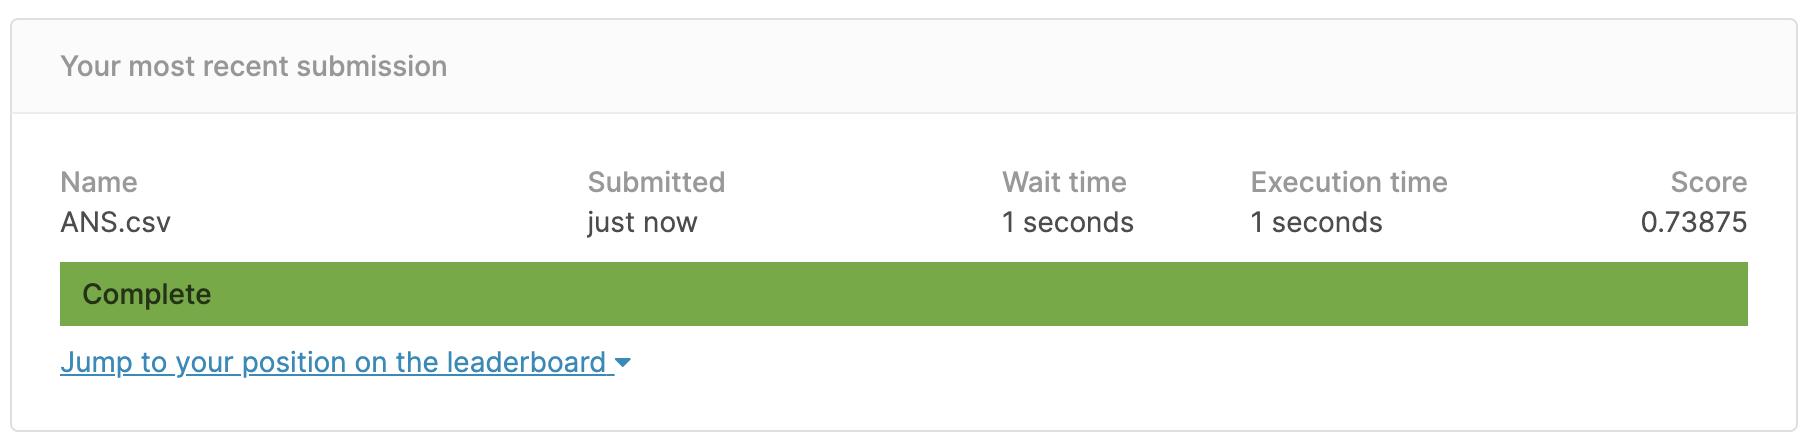
\includegraphics [width=16cm]{download5.png}
\end{figure}


%\section*{References}

\small

%Below is the template of Reference
%[1] Alexander, J.A.\ \& Mozer, M.C.\ (1995) Template-based algorithms for
%connectionist rule extraction. In G.\ Tesauro, D.S.\ Touretzky and T.K.\ Leen
%(eds.), {\it Advances in Neural Information Processing Systems 7},
%pp.\ 609--616. Cambridge, MA: MIT Press.

\end{document}